\documentclass[12pt,amstags,fleqn]{article}

\usepackage{url}

%\usepackage[mathlf,textlf,minionint]{MinionPro} \usepackage[T1]{fontenc} \usepackage{textcomp} \usepackage{amsthm}
\usepackage{amssymb}

\usepackage{amsmath}
\usepackage{amsthm}

\usepackage{xspace}

\theoremstyle{plain}
\newtheorem{theorem}{Theorem}[section]
\newtheorem{lemma}[theorem]{Lemma}
\newtheorem{proposition}[theorem]{Proposition}
\newtheorem{corollary}[theorem]{Corollary}
\newtheorem{conjecture}[theorem]{Conjecture}

\theoremstyle{definition}
\newtheorem{definition}[theorem]{Definition}
\newtheorem{construction}[theorem]{Construction}
\newtheorem{convention}[theorem]{Convention}


% CH: I like Remarks to be in normal font, not italics.
\theoremstyle{definition}
\newtheorem{example}[theorem]{EXAMPLE}
\newtheorem{remark}[theorem]{REMARK}

\newcommand{\Tidentity}{\textnormal{(T1)}\xspace}
\newcommand{\Tcycledisjoint}{\textnormal{(T2)}\xspace}
\newcommand{\Tfpf}{\textnormal{(T3)}\xspace}

\newcommand{\fpf}{fixed-point-free\xspace} 
\newcommand{\fp}{fixed-point\xspace} 
\newcommand{\Fp}{Fixed-point\xspace} 

\newcommand{\Rdisjoint}{\textnormal{(R1)}\xspace}
\newcommand{\RtripA}{\textnormal{(R2)}\xspace}
\newcommand{\RtripB}{\textnormal{(R3)}\xspace}

\newcommand{\Ione}{\textnormal{(I1)}\xspace}
\newcommand{\Itwo}{\textnormal{(I2)}\xspace}

\newcommand{\Ttransitive}{\textnormal{(T4)}\xspace}


\newcommand{\NN}{\mathbb{N}}
\newcommand{\ZZ}{\mathbb{Z}}
\newcommand{\QQ}{\mathbb{Q}}
\newcommand{\CC}{\mathbb{C}}
\newcommand{\CP}{\mathbb{C}\mathbb{P}}
\newcommand{\mov}{\textnormal{Mov}} 
\newcommand{\fix}{\textnormal{Fix}} 

\newcommand{\isomorphic}{\cong}

\newcommand{\darts}{\Omega}

\def\ll{{\textstyle \ast}}
\def\rr{{\scriptscriptstyle \triangle}}

\newcommand{\opa}{\ll} 
\newcommand{\opb}{\rr} 
\newcommand{\opbvar}{\times} 

\newcommand{\blackvertex}{\bullet} 
\newcommand{\whitevertex}{\circ} 
\newcommand{\starvertex}{\star} 

\newcommand{\autotopismgroup}[1]{\textnormal{Aut}(#1)}
\newcommand{\automorphismgroup}[1]{\textnormal{Aut}(#1)}
\newcommand{\underlyingset}{\Omega}

\newcommand{\frattini}{\Phi}    % Frattini subgroup
\newcommand{\sym}{\textnormal{Sym}}    % Symmetric group
\newcommand{\dist}[2]{\textnormal{dist}(#1,\, #2)\xspace}
\newcommand{\metric}[2]{\rho(#1,\, #2)\xspace}
\newcommand{\metricname}{\rho\xspace}
\newcommand{\converges}{\rightarrow\xspace}

\newcommand{\subgroup}{<}
\newcommand{\subgroupeq}{\leq}
\newcommand{\normalsubgroup}{\lhd}
\newcommand{\normalsubgroupeq}{\unlhd}
\newcommand{\subnormal}{\mathop{\normalsubgroupeq \normalsubgroupeq}}

%\def\eq{\operatorname{Eq}\,}
\newcommand{\eq}{\textnormal{Eq}}


\DeclareMathOperator*{\argmax}{arg\, max}
\DeclareMathOperator*{\argmin}{arg\, min}





%%%%%%%%%%%%%%%%%%%%%%%%%%%%%%%%%%%%%%%%%%%%%%%%%%%%%%%%%%
% This stuff is needed to correctly render the metapost
% diagrams depending on whether latex or pdflatex was
% called. Don't change any of it!
\usepackage{ifpdf}

\ifpdf
        \pdfcompresslevel=9
        \usepackage[pdftex]{graphicx}
        %\usepackage{thumbpdf}
        %\usepackage[pdftex,colorlinks,bookmarks,backref]{hyperref}
        %\usepackage[pdftex,backref]{hyperref}
        \DeclareGraphicsRule{*}{mps}{*}{}
\else
        %\usepackage{hyperref}
        %\usepackage[dvips]{graphicx}
        %\usepackage[dvips]{color}
	\usepackage{epsfig}
        \usepackage{graphicx}
        \DeclareGraphicsRule{*}{eps}{*}{}
\fi
%%%%%%%%%%%%%%%%%%%%%%%%%%%%%%%%%%%%%%%%%%%%%%%%%%%%%%%%%%



\title{An enumeration of equilateral triangle dissections}
\author{\Large 
Ale\v s Dr\'apal\footnote{Supported by grant MSM 0021620839}\\
Department of Mathematics \\ Charles University \\ Sokolovsk\'a 83 \\ 186 75 Praha 8 \\ Czech Republic \\
~ \\
Carlo H\"{a}m\"{a}l\"{a}inen\footnote{Supported by Eduard \v Cech center, grant LC505.}  \\
Department of Mathematics \\ Charles University \\ Sokolovsk\'a 83 \\ 186 75 Praha 8 \\ Czech Republic \\
{\texttt carlo.hamalainen@gmail.com}\\
%
}


%\date{}

\begin{document}

\maketitle

\begin{abstract}
We enumerate all dissections of an equilateral triangle into smaller
equilateral triangles. We confirm W.~T. Tutte's claim that the
smallest perfect dissection has size $15$ and we find all perfect
dissections up to size $19$.
\end{abstract}

\section{Introduction}

We are concerned with the following problem: given an equilateral
triangle $\Sigma$, find all dissections of $\Sigma$ into smaller
nonoverlapping equilateral triangles. An example of such a dissection
is shown in Figure~\ref{exDissection}.
Dissections of squares have been studied earlier~\cite{MR0003040}
as well as dissections of squares into right-angled isosceles
triangles~\cite{MR1794696}. Recently, 
Laczkovich\cite{MR1092545} studied tilings of polygons by similar
triangles. The earliest study of dissections of equilateral triangles
into equilateral triangles is by Tutte~\cite{MR0027521}. The problem of
dissecting a triangle is
different to normal tiling problems where the size of the tiles is known
in advance and the tiling area may be infinite.
%%%%%%%%%%%%%%%%%%%%%%%%%%%%%%%%%%%%%%%%%%%%%%%%%%%%%%%%%%%%%%%%%%%%%
\begin{figure}[hbt]
\begin{center}
\includegraphics{output/dissection10_r3_c1}
\end{center}
\caption{An example of an equilateral triangle dissection.}
\label{exDissection}
\end{figure}
%%%%%%%%%%%%%%%%%%%%%%%%%%%%%%%%%%%%%%%%%%%%%%%%%%%%%%%%%%%%%%%%%%%%% 
A naive approach to enumerating dissections is to first fix the sizes and
number of
the dissecting triangles. Observe that in any dissection, some triangles
will be oriented in the same way as the triangle $\Sigma$ (these are the
up-triangles) while the oppositely oriented triangles are the down-triangles.
Let $u_{s}$ and $d_{s}$ be the number of up and down triangles of side
length $s$, respectively. For any down-triangle the horizontal side is
adjacent to the horizontal side of some number of up-triangles. The
up-triangles along the bottom of $\Sigma$ are not adjacent to any
down-triangle. So if the triangle $\Sigma$ has side length $n \in
\mathbb{N}$ then
\begin{equation}\label{eqnSideSum}
\sum_{s} s u_{s} = \sum_{s} s d_{s} + n.
\end{equation}
A triangle with length ${s}$ has height $\sqrt{3}{s}/2$ and so 
the areas sum to give the relation
$\sqrt{3}/{4} \sum_{s} u_{s} 
+
\sqrt{3}/{4} \sum_{s} d_{s} 
= 
\sqrt{3}/{4} n$
which may be rewritten as
\begin{equation}\label{eqnAreaSum}
\sum_{s} u_{s} 
+
\sum_{s} d_{s} 
= 
n.
\end{equation}
Equations~\eqref{eqnSideSum} and \eqref{eqnAreaSum} give:
\begin{equation}\label{eqnAll}
\sum_{s} (1-s) u_{s} + (1+s)d_{s} = 0.
\end{equation}
%A nontrivial dissection with side length $n$ has no triangle of side $n$
%so we may restrict the sum to
%\[
%\sum_{s=1}^{n-1} (1-s) u_{s} + (1+s)d_{s} = 0.
%\]
For small values of $n$ we can solve \eqref{eqnAll} for the permissible
size and number of up and down triangles, and this data may guide an
exhaustive search.
We will consider up and down triangles not to be congruent even
if they are of the same size. A {\em perfect tiling} or
{\em perfect dissection} has no pair of congruent triangles.
Tutte claimed~\cite{MR0003040,MR0027521} that the smallest perfect
dissection has size $15$ (see also~\cite{squaring}).  Unfortunately
solving \eqref{eqnAll} with $n = 15$ is computationally intensive and so
another approach is needed.  Using our enumerative methods we confirm Tutte's
claim and provide all perfect dissections up to size $19$. 


Lines parallel to the outer sides of the main triangle
that are induced by a side
of a dissecting triangle are \emph{dissecting lines}.
For any dissecting line $l$,
the union of all sides of dissecting triangles
that are incident to $l$ forms
one or more contiguous segments. If there are two or more segments,
then on $l$ there exist
two dissecting vertices such that all
triangles in between are cut by the line into two parts. If such
a situation arises for no dissecting line and if no
dissecting vertex is incident to six dissecting triangles,
then we call the dissection \emph{separated}.
We enumerate all isomorphism classes of 
separated dissections up to size $19$. For
the most general class of dissections (including separated and nonseparated) we
provide lower bounds on the number of isomorphism classes up to size
$19$.
%%%%%%%%%%%%%%%%%%%%%%%%%%%%%%%%%%%%%%%%%%%%%%%%%%%%%%%%%%%%%%%%%%%%%
\begin{figure}[hbt]
\begin{center}
%\includegraphics{output-nonsep/dissection10k7_r0_c3.pdf}
\includegraphics{output-nonsep/dissection10k13_r3_c0.pdf}
\end{center}
\caption{A nonseparated dissection.}
\label{nonsepdissection}
\end{figure}
%%%%%%%%%%%%%%%%%%%%%%%%%%%%%%%%%%%%%%%%%%%%%%%%%%%%%%%%%%%%%%%%%%%%% 

\section{Dissections and latin bitrades}

The connection between equilateral triangle dissections and latin
bitrades was first studied in~\cite{aleshamming}. The presentation here
follows~\cite{alesdissections}.  
Consider an equilateral triangle $\Sigma$ that is dissected
into a finite number of equilateral triangles. 
Dissections will be always assumed to be nontrivial so the
number of dissecting triangles is at least four. 
Denote by $a$, $b$ and $c$
the lines induced by the sides of $\Sigma$.
Each side of a dissecting triangle has to be parallel
to one of $a$, $b$, or $c$. If $X$ is a vertex
of a dissecting triangle, then $X$ is a vertex of exactly one,
three or six dissecting triangles. Suppose that there is
no vertex with six triangles and consider triples 
$(u,v,w)$ of lines that are parallel to $a$, $b$ and $c$, respectively,
and meet in  a vertex of a dissecting triangle that is not a vertex
of $\Sigma$. The set of all these triples together with the triple
$(a,b,c)$ will be denoted by $T^\ll$, and by $T^\rr$ we shall
denote the set of all triples $(u,v,w)$ of lines that are yielded 
by sides of a dissecting triangle (where $u$, $v$ and $w$ are again parallel to
$a$, $b$ and $c$, respectively). The following conditions
hold:
\begin{enumerate}
\item[(R1)] Sets $T^\ll$ and $T^\rr$ are disjoint;
\item[(R2)] for all $(p_1,p_2,p_3)\in T^\ll$ and 
all $r,s \in \{1,2,3\}$, $r \ne s$, there exists exactly one
$(q_1,q_2,q_3) \in T^\rr$ with $p_r = q_r$ and $p_s = q_s$; and
\item[(R3)] for all $(q_1,q_2,q_3)\in T^\rr$ and
all $r,s \in \{1,2,3\}$, $r \ne s$, there exists exactly one
$(p_1,p_2,p_3) \in T^\ll$ with $q_r = p_r$ and $q_s = p_s$.
\end{enumerate}

Note that (R2) would not be true if there had existed six dissecting
triangles with a common vertex. Conditions (R1--3) are, in fact, axioms
of a combinatorial object called latin bitrades
\cite[p.~148]{wanlesshandbook}. A bitrade is usually denoted
$(T^{\opa},\, T^{\opb})$. Observe that the bitrade $(T^{\opa},\,
T^{\opb})$ associated with a dissection encodes
qualitative
(structural) information about the segments and intersections of
segments in the dissection. The sizes and number of dissecting triangles
can be recovered by solving a system of equations derived from 
the bitrade (see below).

Dissections are related to a class of latin bitrades with genus~$0$. To
calculate the genus of a bitrade we use a permutation representation to
construct an oriented combinatorial surface~\cite{Dr9,hamalainen2007,ales-geometrical}.
For $r \in \{1,\, 2,\, 3\}$, define the map 
$\beta_r \colon T^{\opb} \rightarrow
T^{\opa}$ where $(a_1,\, a_2,\, a_3) \beta_r = (b_1,\, b_2,\, b_3)$ if and only if
$a_r \neq b_r$
and $a_i = b_i$ for $i \neq r$.
By (R1-3)
% Definition~\ref{defnBitradeA123}
each $\beta_r$ is a bijection.
Then
$\tau_1,\, \tau_2,\, \tau_3\colon T^{\opa} \rightarrow
T^{\opa}$ are defined by
\begin{align}
\tau_1 &= \beta_2^{-1}\beta_3, \qquad
\tau_2 = \beta_3^{-1}\beta_1, \qquad
\tau_3 = \beta_1^{-1}\beta_2. \label{eqnTau}
\end{align}
We refer to
$[\tau_1,\, \tau_2,\, \tau_3]$
as the $\tau_i$ {\em representation}. To get a combinatorial surface
from a bitrade we use the following construction:

%\begin{construction}[$\tau_i$ surface]\label{constructionTauiSurface}
\begin{construction}\label{constructionTauiSurface}
Let $[\tau_1,\, \tau_2,\, \tau_3]$ be the representation for 
a bitrade where the $\tau_i$ act on
the set $\darts$. Define
vertex, directed edge, and face sets by:
\begin{alignat*}{2}
V &= \darts \\
E &= \{ (x,y) \mid x \tau_1 = y \} \cup \{ (x,y) \mid x \tau_2 = y \} \cup \{ (x,y) \mid x \tau_3 = y \} \\
F &= \{ (x,y,z) \mid \text{ $x \tau_1 = y$, $y \tau_2 = z$, $z \tau_3 = x$} \} \\
  & \qquad \cup \{ (x_1,\, x_2,\, \dots,\, x_r) \mid \text{ $(x_1,\,
x_2,\, \dots,\, x_r)$ is a cycle of $\tau_1$ } \} \\
  & \qquad \cup \{ (x_1,\, x_2,\, \dots,\, x_r) \mid \text{ $(x_1,\,
x_2,\, \dots,\, x_r)$ is a cycle of $\tau_2$ } \} \\
  & \qquad \cup \{ (x_1,\, x_2,\, \dots,\, x_r) \mid \text{ $(x_1,\,
x_2,\, \dots,\, x_r)$ is a cycle of $\tau_3$ } \}
\end{alignat*}
where $(x_1,\, x_2,\, \dots,\, x_k)$ denotes a face with $k$~directed edges
$(x_1,\, x_2)$, $(x_2,\, x_3)$, $\dots$,
$(x_{k-1},\, x_k)$, $(x_k,\, x_1)$ for vertices
$x_1,\, \dots,\, x_k$.

The first set in the definition of $F$ is the set of {\em triangular
faces}, while the other three are the {\em $\tau_i$ faces}.
Assign triangular faces a positive (anticlockwise) orientation, and
assign
$\tau_i$ faces negative (clockwise) orientation. Now glue the faces
together where they share a common directed edge $x \tau_i = y$,
ensuring that edges come together with opposite orientation.
%(see
%Construction~\ref{constructionSAPtoMap} and 
%Example~\ref{exGluingFaces} for another example of this type of gluing process).
\end{construction}

%Theorem~\ref{theoremMapRotation} ensures that the construction does
%produce a combinatorial surface.
The orientation of a triangular face is
shown in Figure~\ref{figTwoOrientations} along with the orientation for
a $\tau_i$ face. For the sake of concreteness we have illustrated a
$6$-cycle face due to a $6$-cycle of $\tau_1$. 
Figure~\ref{figDrapalRotationScheme} shows
the rotation scheme for an arbitrary vertex in the surface.
%%%%%%%%%%%%%%%%%%%%%%%%%%%%%%%%%%%%%%%%%%%%%%%%%%%%%%%%%%%%%%%%%%%%%
\begin{figure}[htb]
\begin{center}
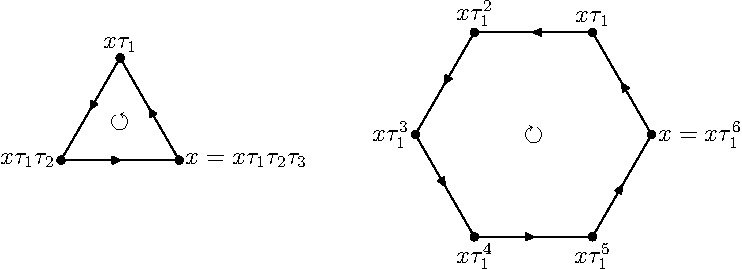
\includegraphics{drRotationScheme-1.pdf}
\end{center}
\caption{Orienting faces in the combinatorial surface.}
\label{figTwoOrientations}
\end{figure}
%%%%%%%%%%%%%%%%%%%%%%%%%%%%%%%%%%%%%%%%%%%%%%%%%%%%%%%%%%%%%%%%%%%%% 
%%%%%%%%%%%%%%%%%%%%%%%%%%%%%%%%%%%%%%%%%%%%%%%%%%%%%%%%%%%%%%%%%%%%%
\begin{figure}[htb]
\begin{center}
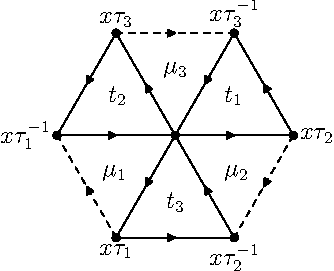
\includegraphics{drRotationScheme-2.pdf}
\end{center}
\caption{Rotation scheme for the combinatorial surface. Dashed
lines represent one or more edges, where $\mu_i$ is a cycle of $\tau_i$.
The vertex in the centre is $x$.}
\label{figDrapalRotationScheme}
\end{figure}
%%%%%%%%%%%%%%%%%%%%%%%%%%%%%%%%%%%%%%%%%%%%%%%%%%%%%%%%%%%%%%%%%%%%% 

For a bitrade $T = (T^{\opa},\, T^{\opb})$ with representation 
$[\tau_1,\, \tau_2,\, \tau_3]$
on the set $\darts$,
% = \mov(\tau_1) \cup \mov(\tau_2) \cup \mov(\tau_3)$,
define
$\text{order}(T)  = z(\tau_1) + z(\tau_2) + z(\tau_3)$, the total number
of cycles, and
$\text{size}(T) = \left| \darts \right|$, the total number of points 
that the $\tau_i$ act on. 
By some basic counting arguments we find that there are 
$\text{size}(T)$ vertices, $3 \cdot \text{size}(T)$ edges, and 
$\text{order}(T) + \text{size}(T)$ faces. Then Euler's formula
$V-E+F=2-2g$ gives
\begin{equation}\label{eqnDrapalGenus}
\text{order}(T) = \text{size}(T) + 2 - 2g
\end{equation}
where $g$ is the genus of the combinatorial surface. We say that
the bitrade $T$ has genus $g$.
A {\em spherical bitrade} has genus~$0$.

\begin{example}\label{exspherical}
The following bitrade is spherical:
\begin{align*}
T^{\opa} = 
\begin{array}{|c||c|c|c|c|c|}
\hline
\opa & 0 & 1 & 2 & 3 & 4\\
\hline
 \hline 0 & 0 & ~ & 2 & ~ & 4\\
 \hline 1 & ~ & ~ & ~ & 4 & 2\\
 \hline 2 & 1 & 3 & 0 & 2 & ~\\
 \hline 3 & 4 & 1 & ~ & 3 & ~\\
 %\hline 4 & ~ & ~ & ~ & ~ & ~ \\
\hline
\end{array}
& \quad & 
T^{\opb} = 
\begin{array}{|c||c|c|c|c|c|}
\hline
\opb & 0 & 1 & 2 & 3 & 4\\
\hline
 \hline 0 & 4 & ~ & 0 & ~ & 2\\
 \hline 1 & ~ & ~ & ~ & 2 & 4\\
 \hline 2 & 0 & 1 & 2 & 3 & ~\\
 \hline 3 & 1 & 3 & ~ & 4 & ~\\ 
%\hline 4 & ~ & ~ & ~ & ~ & ~\\
\hline
\end{array}
%\label{eqnsphericalbitrade}
\end{align*}
Here, the $\tau_i$ representation is
\begin{align*}
\tau_1 &= (000, 022, 044)(134, 142) (201,213,232,220) (304,333,311) \\
\tau_2 &= (000,304,201)(213,311)(022,220)(134,232,333)(044,142) \\
\tau_3 &= (000,220)(201,311)(022,232,142)(213,333)(044,134,304)
\end{align*}
where the triples $ijk$ refer to entries $(i,j,k) \in T^{\opa}$.
\end{example}



%\begin{theorem}[{Dr\a'apal~\cite{Dr9}}]\label{theoremDrapalTauStructure}
%A bitrade $(T^{\opa},\, T^{\opb})$ is equivalent (up to isotopism) to three
%permutations $\tau_1$, $\tau_2$, $\tau_3$ acting on a set $\darts$
%satisfying \Tidentity, \Tcycledisjoint, and \Tfpf. 
%If \Ttransitive is also satisfied then the bitrade is indecomposable.
%\end{theorem}

We will generally assume that a bitrade is {\em separated}, that is,
each row, column, and symbol is in bijection with a cycle of $\tau_1$,
$\tau_2$, and $\tau_3$, respectively.

We now describe how to go from a separated spherical latin bitrade to a
triangle dissection (for more details see~\cite{alesdissections}).  
Let $T= (T^\ll, T^\rr)$ be a latin bitrade. It is natural to have
different unknowns for rows, columns and symbols, and so we assume
that $a_i \ne b_j$ whenever $(a_1,a_2,a_3)$, $(b_1,b_2,b_3) \in T^\ll$
and $1 \le i < j \le 3$.  (If the condition is violated,  then $T$
can be replaced by an isotopic bitrade for which it is satisfied.)
Fix a triple $a = (a_1,a_2,a_3) \in T^\ll$ and form the set of equations
$\eq(T)$ consisting of
$a_1=0$, $a_2=0$, $a_3 =1$
and 
$b_1+b_2 = b_3$  if $(b_1,b_2,b_3) \neq (a_1,a_2,a_3)$
and $(b_1,b_2,b_3) \in T^\ll$.
The theorem below shows that if $T$ is a spherical latin
bitrade then $\eq(T, a)$ always has a unique solution in the rationals.

Write
$\bar r_i$,
$\bar c_j$,
$\bar s_k$
for the solutions in $\eq(T, a)$ for row variable $r_i$, column variable
$c_j$, and symbol variable $s_k$, respectively. We say that 
a solution to $\eq(T, a)$ is {\em separated} if 
$\bar r_i \neq \bar r_{i'}$ whenever $i \neq i'$ (and similar for
columns and symbols).

For each entry $c = (c_1,c_2,c_3) \in T^\rr$ we form the triangle
$\Delta(c,a)$ which is bounded by the lines
$y = \bar c_1$,
$x = \bar c_2$,
$x + y = \bar c_3$.
%A dissection is {\em separated} if there is no (interior) vertex of
%degree~$6$.
A dissection with $m$ vertices has size $m-2$. A separated dissection 
with $m$ vertices corresponds to a separated spherical bitrade
$(T^{\opa},\, T^{\opb})$ where $\left| T^{\opa} \right| = m-2$.  
The main result of~\cite{alesdissections} is the following theorem:

\begin{theorem}[\cite{alesdissections}]\label{sepdissections}
Let $T=(T^\ll, T^\rr)$ be a spherical latin bitrade,
and suppose that $a=(a_1,a_2,a_3) \in T^\ll$ is a triple such
that the solution to $\eq(T,a)$ is separated. Then the set
of all triangles $\Delta(c,a)$, $c \in T^\rr$, dissects the triangle
$\Sigma = \{(x,y);$ $x\ge 0$, $y\ge 0$ and $x+y \le 1\}$. This
dissection is separated.
\end{theorem}

An equilateral dissection can be obtained by applying the transformation
$(x,y) \mapsto (y/2 + x, \sqrt 3 y/2)$.

\begin{example}
For example, consider the following spherical bitrade 
$(T^{\ll},\, T^{\rr})$:  \\ 
\[
T^{\ll} = 
\begin{array}{|c||c|c|c|c|c|}
\hline \ll & c_0 & c_1 & c_2 & c_3 & c_4\\
\hline \hline r_0 & s_4 & ~ & s_0 & ~ & s_2\\
\hline r_1 & ~ & ~ & ~ & s_2 & s_4\\
\hline r_2 & s_0 & s_1 & s_2 & s_3 & ~\\
\hline r_3 & s_1 & s_3 & ~ & s_4 & ~\\
\hline \end{array} 
\quad 
T^{\rr} = 
\begin{array}{|c||c|c|c|c|c|}
\hline \rr & c_0 & c_1 & c_2 & c_3 & c_4\\
\hline \hline r_0 & s_0 & ~ & s_2 & ~ & s_4\\
\hline r_1 & ~ & ~ & ~ & s_4 & s_2\\
\hline r_2 & s_1 & s_3 & s_0 & s_2 & ~\\
\hline r_3 & s_4 & s_1 & ~ & s_3 & ~\\
\hline \end{array}
\label{eqnsphericalbitrade}
\]

Let $a = (a_1,a_2,a_3) = (r_0,c_0,s_4)$. Then the system of equations
$\textnormal{Eq}(T, a)$ has the solution
\begin{align*}
\bar r_0 &= 0,\, \bar r_1 = 2/7,\, \bar r_2 = 5/14,\, \bar r_3 = 4/7 \\
\bar c_0 &= 0,\, \bar c_1 = 3/14,\, \bar c_2 = 5/14,\, \bar c_3 = 3/7,\, \bar c_4 = 5/7 \\
\bar s_0 &= 5/14,\, \bar s_1 = 4/7,\, \bar s_2 = 5/7,\, \bar s_3 = 11/14,\, \bar s_4 = 1.
\end{align*}
The dissection is shown in Figure~\ref{fg2}.
 Entries of
$T^{\rr}$ correspond to triangles in the dissection. For example,
$(r_0,c_0,s_0) \in T^{\rr}$ is the triangle bounded by the lines
$y = \bar r_0 = 0$, 
$x = \bar c_0 = 0$, 
$x+y = \bar s_0 = 5/14$ while 
$(r_1,c_3,s_2) \in T^{\ll}$ corresponds to the intersection of the
lines
$y = \bar r_1 = 2/7$, 
$x = \bar c_3 = 3/7$, 
$x+y = \bar s_2 = 5/7$.
\end{example}

\begin{figure}[htbp]
\begin{center}
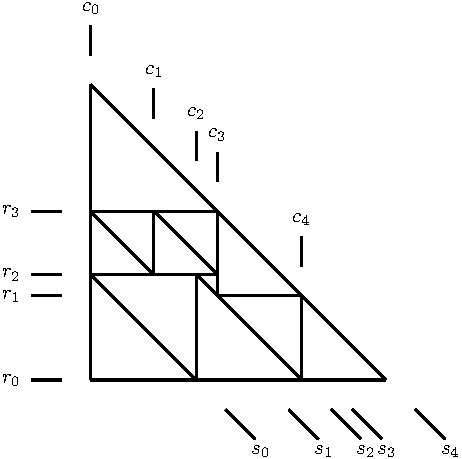
\includegraphics[scale=0.75]{dissection31}
\end{center}
\caption{Dissection for a spherical bitrade. The labels $r_i$, $c_j$,
$s_k$, refer to lines $y = \bar r_i$,
$x = \bar c_j$,
$x+y = \bar s_k$, respectively. The trade $T^{\opa}$ has $12$ entries
and the dissection has $12 + 2 = 14$ vertices.
Applying the transformation $(x,y) \mapsto (y/2 + x, \sqrt 3 y/2)$ gives
an equilateral dissection.}
\label{fg2}
\end{figure} 

\begin{remark}
Suppose that the dissection $\Sigma$ has no vertex of degree $6$.
Pick a vertex $X$ of degree~$4$. If we
move to the right along the row segment to the next vertex $X'$ then we
have $X \tau_1 = X'$. Similarly, moving along the diagonal segments
gives the action of $\tau_2$ and $\tau_3$. If we identify the three vertices of degree $2$
then the dissection encodes, geometrically,
the permutation representation of the bitrade.

If a dissection has a vertex of degree~$6$ then the dissecting triangles
do not (uniquely) define a partial latin square and hence do not encode
a latin bitrade. However, we can recover a separated
bitrade by the following procedure. For each vertex $X$ of degree~$6$,
choose one segment (say, the $r_i$ segment) to stay fixed. Then for the $c_j$
and $s_k$ segments, label the column segment below $X$ with a new name $c'$
and label the symbol segment below $X$ with a new name $s'$. For example,
the centre vertex in Figure~\ref{figsixway} results in the new labels
$c_3$ and $s_3$. The resulting separated bitrade is:
\[ T^{\ast},\, T^{\triangle} =\begin{array}{|c||c|c|c|c|}
\hline \ast & c_0 & c_1 & c_2 & c_3\\
\hline \hline r_0 & s_2 & ~ & s_3 & s_0\\\hline r_1 & s_0 & s_1 & s_2 & s_3\\\hline r_2 & s_1 & s_2 & ~ & ~\\\hline\end{array}\phantom{x}\begin{array}{|c||c|c|c|c|}
\hline \triangle & c_0 & c_1 & c_2 & c_3\\
\hline \hline r_0 & s_0 & ~ & s_2 & s_3\\\hline r_1 & s_1 & s_2 & s_3 & s_0\\\hline r_2 & s_2 & s_1 & ~ & ~\\\hline\end{array}\]
This procedure works for any number of vertices of degree~$6$, as long
as care is taken to only relabel column or symbol segments below a
vertex of degree~$6$ and not to relabel a segment more than
once.\footnote{For a concrete implementation, see 
\texttt{generate\_bitrade\_via\_geometric\_data} in\\
\texttt{triangle\_dissections.py} in \cite{dissections}}
\end{remark}
%%%%%%%%%%%%%%%%%%%%%%%%%%%%%%%%%%%%%%%%%%%%%%%%%%%%%%%%%%%%%%%%%%%%%
\begin{figure}[hbt]
\begin{center}
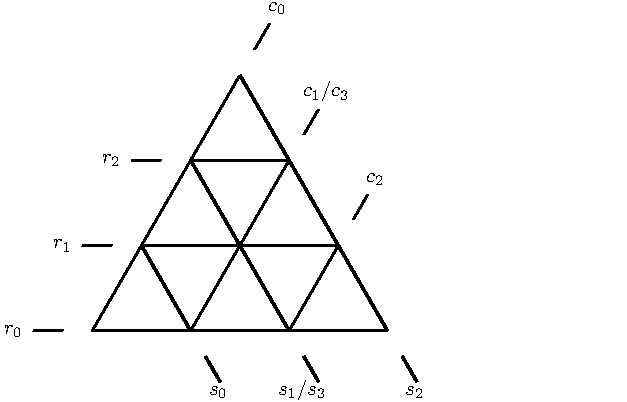
\includegraphics{sixway.pdf}
\end{center}
\caption{A dissection with a vertex of degree $6$.}
\label{figsixway}
\end{figure}
%%%%%%%%%%%%%%%%%%%%%%%%%%%%%%%%%%%%%%%%%%%%%%%%%%%%%%%%%%%%%%%%%%%%% 

\section{Computational results}

Cavenagh and Lisonek~\cite{planareulerian} showed that spherical
bitrades are equivalent to planar Eulerian triangulations. To enumerate
separated triangle dissections we
use plantri~\cite{plantri} to enumerate all planar
Eulerian triangulations up to a specified size. We wrote a 
plugin~\cite{code} to output the equivalent spherical latin bitrade
$(U^{\opa}, U^{\opb})$ for each triangulation. For each such
$(U^{\opa},U^{\opb})$ we find all
separated solutions $\eq(T, a)$ for all $a \in T^{\opa}$ and compute each
dissection (in practise this is a list of triangles $\Delta(c,a)$ for
each $c = (c_1,c_2,c_3) \in T^{\rr}$).
To filter out isomorphic dissections we apply all six elements of
the symmetry group for a unit-side equilateral triangle (identity, two rotations,
and three reflections). The {\em canonical signature} of a dissection 
$\Delta(T,a)$ is
the ordered list $[(x,y) \mid (x,y) \textnormal{ is a
vertex of $\Delta(T,a)$}]$. We repeat the whole process for the bitrade $(U^{\opb},U^{\opa})$
because there are spherical latin bitrades where
$(U^{\opa},U^{\opb})$ is not isomorphic to $(U^{\opb},U^{\opa})$.  
Throughout we use the SymPy package~\cite{sympy} to perform
exact symbolic arithmetic so that the canonical form of a dissection is
not affected by round-off error and other floating point issues.


\subsection{Separated dissections}

Using Theorem~\ref{sepdissections}
we have enumerated the number of isomorphism classes of separated
dissections of size $n$. We also record $A(n,k)$, the number of dissections of 
size $n$ with automorphism group of order $k$.

\begin{center}
\begin{tabular}{|c|c|c|c|c|c|}
\hline $n$ & \# dissections & $A(n,1)$ & $A(n,2)$ & $A(n,3)$ & $A(n,6)$ \\
\hline
\hline 4 & 1 & 0 & 0 & 0 & 1 \\
\hline 6 & 1 & 0 & 1 & 0 & 0 \\
\hline 7 & 2 & 0 & 1 & 0 & 1 \\
\hline 8 & 3 & 2 & 1 & 0 & 0 \\
\hline 9 & 8 & 4 & 4 & 0 & 0 \\
\hline 10 & 20 & 15 & 4 & 0 & 1 \\
\hline 11 & 55 & 47 & 8 & 0 & 0 \\
\hline 12 & 161 & 146 & 15 & 0 & 0 \\
\hline 13 & 478 & 460 & 17 & 0 & 1 \\
\hline 14 & 1496 & 1459 & 37 & 0 & 0 \\
\hline 15 & 4804 & 4746 & 58 & 0 & 0 \\
\hline 16 & 15589 & 15506 & 82 & 0 & 1 \\
\hline 17 & 51377 & 51223 & 154 & 0 & 0 \\
\hline 18 & 172162 & 171923 & 239 & 0 & 0 \\
\hline 19 & 583810 & 583426 & 383 & 0 & 1 \\
\hline
\end{tabular}
\end{center}

\subsection{Perfect dissections}

%Equilateral triangles can tile in an up or down direction, depending on
%whether the vertex opposite the triangle's horizontal side is above or
%below the horizontal side. If these triangles are considered to be
%different since they are not congruent (even though they are of the same
%size) then we get the notion of a {\em perfect tiling} or {\em perfect
%dissection}~\cite{squaring}.

Using our enumeration code we can confirm W.~T. Tutte's
claim~\cite{MR0003040,MR0027521}
that the smallest perfect dissection has size $15$ (see
Figure~\ref{figPerfect15}).
The perfect dissections of size $16$ and $17$ are shown in
Figures~\ref{figPerfect16} and \ref{figPerfect17}.
%
\begin{figure}[htbp]
\begin{center}
\includegraphics{perfect_dissection_size15_595_r5_c3.pdf}\includegraphics{perfect_dissection_size15_595_r5_c4.pdf}
\end{center}
\caption{The two perfect dissections of size $15$ (with $15+2 = 17$
vertices).}
\label{figPerfect15}
\end{figure}
%
\begin{figure}[htbp]
\begin{center}
\includegraphics{perfect_dissection_size16_3073_r2_c3.pdf}\includegraphics{perfect_dissection_size16_3073_r2_c5.pdf}
\end{center}
\caption{The two perfect dissections of size $16$.}
\label{figPerfect16}
\end{figure}
%
\begin{figure}[htbp]
\begin{center}
\includegraphics{perfect_dissection_size17_12169_r1_c6.pdf}\includegraphics{perfect_dissection_size17_12169_r5_c6.pdf}
\includegraphics{perfect_dissection_size17_3091_r2_c4.pdf}\includegraphics{perfect_dissection_size17_3091_r3_c0.pdf}
\includegraphics{perfect_dissection_size17_3095_r0_c2.pdf}\includegraphics{perfect_dissection_size17_3095_r1_c3.pdf}
\end{center}
\caption{The six perfect dissections of size $17$.}
\label{figPerfect17}
\end{figure}
%
The perfect dissections of size $15$,
$16$,
$17$,
$18$, and
$19$ are available in PDF format~\cite{dissections}.
The following table summarises the known number of isomorphism classes
of perfect dissections:

\begin{center}
\begin{tabular}{|c|c|}
\hline $n$ & \# perfect dissections \\
\hline
\hline 15 & 2 \\
\hline 16 & 2 \\
\hline 17 & 6 \\
\hline 18 & 23 \\
\hline 19 & 64 \\
\hline
\end{tabular}
\end{center}

\subsection{Lower bounds on all dissections}

If we drop the condition that the solution to $\eq(T, a)$ is separated
then we obtain the following conjecture, which has been verified by
computer for all spherical bitrades up to size $20$:
 
\begin{conjecture}\label{mainconjecture}
Let $T=(T^\ll, T^\rr)$ be a spherical latin bitrade. Then for 
any $a=(a_1,a_2,a_3) \in T^\ll$,
the solution to $\eq(T,a)$ determines a set of 
triangles $\Delta(c,a)$, $c \in T^\rr$ that dissects the triangle
$\Sigma = \{(x,y);$ $x\ge 0$, $y\ge 0$ and $x+y \le 1\}$. This
dissection may not be separated.
\end{conjecture}

It is important to note that the resulting dissection from a
nonseparated solution may be smaller than a separated solution.



To enumerate nonseparated dissections we have to consider nonseparated
solutions to $\eq(T,a)$. This in turn means that a particular separated
dissection may only arise from a larger bitrade. Dissections are
assumed to be nontrivial so on each side there must be a vertex, and
each such vertex has degree $4$. So in any dissection with $n$ vertices
there are at most $n - 4$ vertices of degree $6$. The three outer
vertices correspond to one entry in $T^{\opa}$ of the source bitrade
$(T^{\opa},\, T^{\opb})$. The three side vertices correspond to three
distinct entries of $T^{\opa}$. Finally, the $n-4$ vertices of degree
$6$ correspond to at most $2(n-4)$ entries of $T^{\opa}$. Hence
$\left| T^{\opa} \right| \leq 4 + 2(n-4) = 2n - 4$.
For example, one of the separated dissections on $8$ points is derived
from a bitrade of size $9$.

Since we have enumerated all separated dissections up to size $19$, we
are able to use Conjecture~\ref{mainconjecture} to enumerate the exact
number of separated and nonseparated dissections up to size $9$ (with
$9+2=11$ vertices) and we can give lower bounds up to size $19$.

\begin{center}
\begin{tabular}{|c|c|}
\hline $n$ & \# dissections \\
\hline
\hline 4 & 1 \\
\hline 6 & 1 \\
\hline 7 & 2 \\
\hline 8 & 4 \\
\hline 9 & 9 \\
\hline 10 & $\geqslant$ 24 \\
\hline 11 & $\geqslant$ 71 \\
\hline 12 & $\geqslant$ 206 \\
\hline 13 & $\geqslant$ 636 \\
\hline 14 & $\geqslant$ 2043 \\
\hline 15 & $\geqslant$ 6679 \\
\hline 16 & $\geqslant$ 22260 \\
\hline 17 & $\geqslant$ 75002 \\
\hline 18 & $\geqslant$ 251092 \\
\hline 19 & $\geqslant$ 732847 \\
\hline
\end{tabular}
\end{center}

\subsection{Other observations}

There exist bitrades of size $n \geq 10$ for which there is no
separated dissection of size $n$. The following table shows a sample
of these bitrades, giving the sizes of all possible dissections for
the particular bitrade of size $n$.

\begin{center}
\begin{tabular}{|c|l|}
\hline
$n$ & size of possible dissections \\
\hline
\hline 10 & 4, 7  \\
\hline 12 & 4, 7, 8, 9  \\
\hline 12 & 4, 9, 11  \\
\hline 12 & 4, 11  \\
\hline 12 & 6, 9  \\
\hline 12 & 9  \\
\hline 12 & 11  \\
\hline 13 & 4, 7  \\
\hline 13 & 4, 7, 9, 10  \\
\hline 13 & 4, 7, 10  \\
\hline 13 & 4, 9, 10, 12  \\
\hline 13 & 4, 11, 12  \\
\hline 13 & 9, 10, 12  \\
\hline 13 & 10, 11  \\
\hline
\end{tabular}
\end{center}

A {\em trivial dissection} has triangles of only one size. Apart from
$n = 4$, all trivial dissections are nonseparated.  The following
table lists lower bounds on the number of bitrades that give rise to
the (unique) separated dissection of size $n$ (naturally we allow for
nonseparated solutions to find these trivial dissections).

\begin{center}
\begin{tabular}{|c|l|}
\hline
$n$ & lower bound on number of source bitrades \\
\hline
\hline 4 & 2380591 \\
\hline 8 & 111890 \\
\hline 13 & 1321 \\ 
\hline
\end{tabular}
\end{center}

For each size $n$ we collect examples of dissections with the largest
relative difference in size between the largest and smallest triangle in
the dissection. In all cases the smallest triangle has size $1$ and the
largest triangle  is given in the second column of the table below:

\begin{center}
\begin{tabular}{|c|c|c|c|}
\hline
$n$ & size of largest triangle \\
\hline
\hline 4 & 1 \\
\hline 6 & 2 \\
\hline 7 & 2 \\
\hline 8 & 3 \\
\hline 9 & 4 \\
\hline 10 & 5 \\
\hline 11 & 7 \\
\hline 12 & 9 \\
\hline 13 & 12 \\
\hline 14 & 16 \\
\hline 15 & 21 \\
\hline 16 & 28 \\
\hline 17 & 37 \\
\hline 18 & 49 \\
\hline 19 & 67 \\
\hline 20 & 91 \\
\hline
\end{tabular}
\end{center}

The dissections that give rise to these maximum ratios are shown below
(sorted by dissection size $n$):

\begin{center}
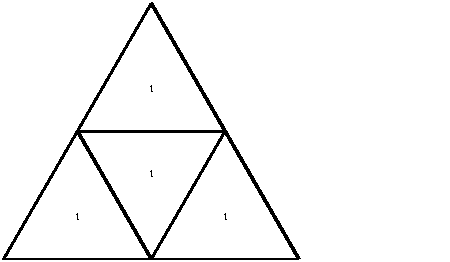
\includegraphics{max_relative_size_4.pdf}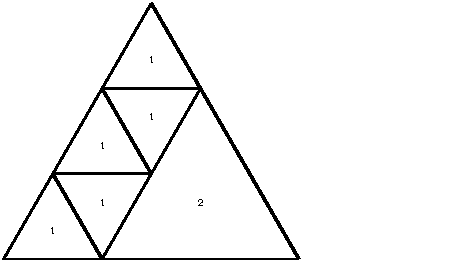
\includegraphics{max_relative_size_6.pdf}
\end{center}
\begin{center}
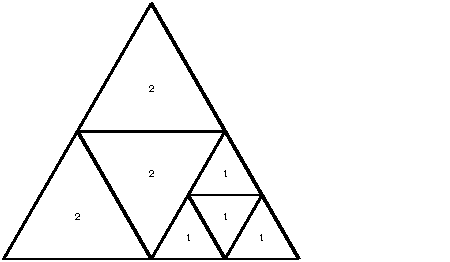
\includegraphics{max_relative_size_7.pdf}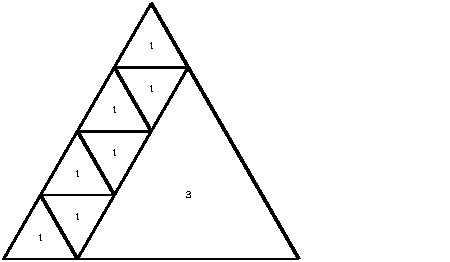
\includegraphics{max_relative_size_8.pdf}
\end{center}
\begin{center}
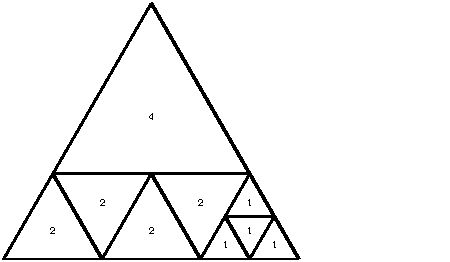
\includegraphics{max_relative_size_9.pdf}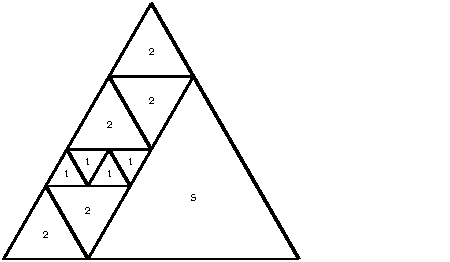
\includegraphics{max_relative_size_10.pdf}
\end{center}
\begin{center}
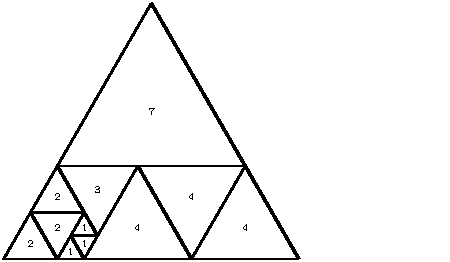
\includegraphics{max_relative_size_11.pdf}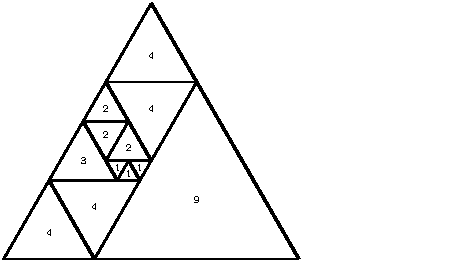
\includegraphics{max_relative_size_12.pdf}
\end{center}
\begin{center}
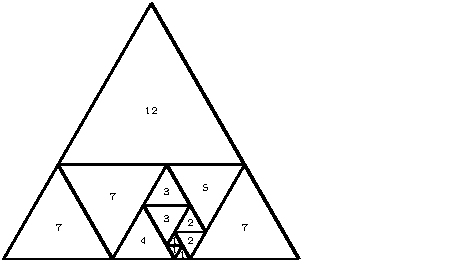
\includegraphics{max_relative_size_13.pdf}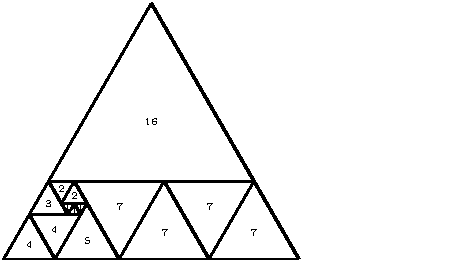
\includegraphics{max_relative_size_14.pdf}
\end{center}
\begin{center}
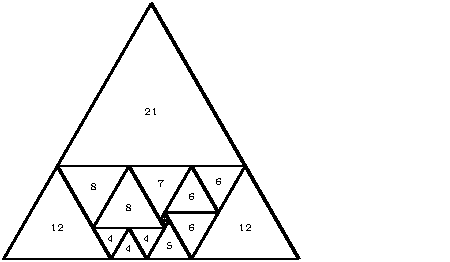
\includegraphics{max_relative_size_15.pdf}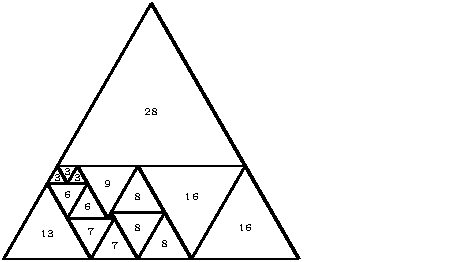
\includegraphics{max_relative_size_16.pdf}
\end{center}
\begin{center}
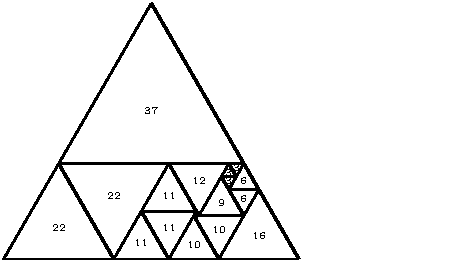
\includegraphics{max_relative_size_17.pdf}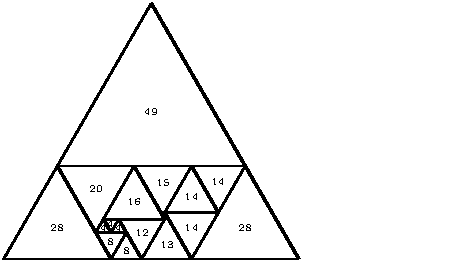
\includegraphics{max_relative_size_18.pdf}
\end{center}
\begin{center}
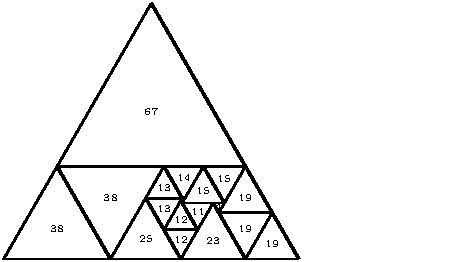
\includegraphics{max_relative_size_19.pdf}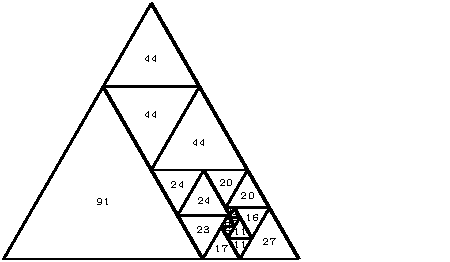
\includegraphics{max_relative_size_20.pdf}
\end{center}

\clearpage

\bibliographystyle{plain}
\bibliography{unique_dissections}

\clearpage

\section*{Appendix A: Separated triangle dissections}

Here we present representatives of the isomorphism classes of separated triangle
dissections of size $n \in \{4, 6, 7, 8, 9, 10 \}$.

\input{data_unique_dissections.tex}

\section*{Appendix B: Nonseparated triangle dissections}

Here we present the known nonseparated triangle dissections of size at
most $10$, up to isomorphism.

\subsection*{$n = 8$}

\begin{center}
\includegraphics{output-nonsep/dissection8k1_r0_c0.pdf}
\end{center}

\subsection*{$n = 9$}

\begin{center}
\includegraphics{output-nonsep/dissection9k0_r3_c1.pdf}
\end{center}

\subsection*{$n = 10$}

\begin{center}
\includegraphics{output-nonsep/dissection10k1_r1_c2.pdf}\includegraphics{output-nonsep/dissection10k6_r0_c2.pdf}
\end{center}
\begin{center}
\includegraphics{output-nonsep/dissection10k7_r0_c3.pdf}\includegraphics{output-nonsep/dissection10k13_r3_c0.pdf}
\end{center}


\end{document}
\clearpage



\section{Introduction}

A {\em latin bitrade} $(T^{\opa},\, T^{\opb})$ is a pair of partial
latin squares which are disjoint, occupy the same set of non-empty
cells, and whose corresponding rows and columns contain the same set
of entries. One of the earliest studies of latin bitrades appeared 
in~\cite{DrKe1}, where they are referred to as {\em exchangeable partial
groupoids}. Latin bitrades are prominent in the study of 
{\em critical sets}, which are minimal defining sets of latin squares
(\cite{BaRe2},\cite{codose},\cite{Ke2}) and the intersections
between latin squares (\cite{Fu}). A genus may be associated to a latin
bitrade, and those of genus zero are known as {\em spherical} latin
bitrades.

Spherical latin bitrades, that is latin bitrades with genus zero, may be
associated with dissections of equilateral triangles into smaller
equilateral triangles. Using plantri~\cite{plantri} and our own code~\cite{code}, \cite{dissections}
we are able to
enumerate all equilateral triangle dissections up to size $19$ that
contain no vertex of degree~$6$ (these are known as separated
dissections), and provide a lower bound on all
equilateral triangle dissections up to size $19$ that may include
vertices of degree~$6$.

\section{Latin bitrades}

A {\em partial latin square} $P$ of order $n > 0$ is an 
$n \times n$ array where each $e \in \{ 0, 1, \dots, n-1 \}$
appears at most once in each row, and at most once in each column.
A {\em latin square} $L$ of order $n > 0$ is an
$n \times n$ array where each $e \in \{ 0, 1, \dots, n-1 \}$
appears exactly once in each row, and exactly once in each column.
It is convenient to use setwise notation to refer to entries
of a (partial) latin square, and we
write $(i,j,k) \in P$ if and only if symbol $k$ appears in the
intersection of row $i$ and column $j$ of $P$.
In this manner, $P \subseteq A_1 \times A_2 \times A_3$ for finite sets
$A_i$, each of size $n$.
It is also convenient to interpret a (partial) latin square as a multiplication
table for a (partial) binary operator $\opa$, writing
$i \opa j = k$ if and only if $(i,j,k) \in T = T^{\opa}$.

\begin{definition}\label{defnBitradeA123}
Let $T^{\opa}$, $T^{\opb} \subseteq A_1 \times A_2 \times A_3$ be
two partial latin squares. Then $(T^{\opa},\, T^{\opb})$ is a {\em
bitrade} if the following three conditions are satisfied:
\begin{itemize}

\item[\Rdisjoint] $T^{\opa} \cap T^{\opb} = \emptyset$;

\item[\RtripA] for all $(a_1,\, a_2,\, a_3) \in T^{\opa}$ and all $r$,
$s \in \{1,\, 2,\, 3\}$,
$r \neq s$, there exists a unique $(b_1,\, b_2,\, b_3) \in T^{\opb}$
such that $a_r=b_r$ and $a_s=b_s$;

\item[\RtripB] for all $(a_1,\, a_2,\, a_3) \in T^{\opb}$ and all $r$,
$s \in \{1,\, 2,\, 3\}$,
$r \neq s$, there exists a unique $(b_1,\, b_2,\, b_3) \in T^{\opa}$
such that $a_r=b_r$ and $a_s=b_s$.

\end{itemize}
\end{definition}

Conditions~\RtripA and \RtripB imply that each row (column) of
$T^{\opa}$ contains the same subset of $A_3$ as the corresponding row
(column) of $T^{\opb}$.
A bitrade $(T^{\opa},\, T^{\opb})$ is {\em indecomposable\/}
if whenever $(U^{\opa},\,U^{\opb})$ is a bitrade such that
$U^{\opa}\subseteq
T^{\opa}$ 
and
$U^{\opb}\subseteq   
T^{\opb}$, then 
$(T^{\opa},\, T^{\opb})=  
(U^{\opa},\, U^{\opb})$.  
Bijections $A_i \rightarrow A'_i$, for $i = 1$, $2$, $3$, give an 
{\em isotopic} bitrade, and permuting each $A_i$ gives an {\em
autotopism}. We refer to the bijections
$\{A_1 \rightarrow A'_1,
A_2 \rightarrow A'_2,
A_3 \rightarrow A'_3\}$ as an {\em isotopism}.


We write $\mov(\pi)$ for the set of points that the (finite) permutation
$\pi$ acts on.

\begin{definition}\label{defnT1234}
Let $\tau_1$, $\tau_2$, $\tau_3$ be (finite) permutations
and let $\darts = \mov(\tau_1) \cup \mov(\tau_2) \cup \mov(\tau_3)$.  
Define four properties:
\begin{enumerate}

\item[\Tidentity] $\tau_1 \tau_2 \tau_3 = 1$;

%\item[\Tcycledisjoint] an orbit $\rho$ of $\tau_i$ has at most one point in common
%with an orbit $\mu$ of $\tau_j$, where $1 \leq i < j \leq 3$;
\item[\Tcycledisjoint] if $\rho_i$ is a cycle of $\tau_i$
and $\rho_j$ is a cycle of $\tau_j$
then $\left| \mov(\rho_i) \cap \mov(\rho_j) \right| \leq 1$,
for any $1 \leq i < j \leq 3$;

\item[\Tfpf] each $\tau_i$ is \fpf;

\item[\Ttransitive] the group $\langle \tau_1,\, \tau_2,\, \tau_3 \rangle$ is
transitive on $\darts$.
\end{enumerate}

\end{definition}

Letting $A_i$ be the set of cycles of $\tau_i$, we have the
following theorem, which relates
Definition~\ref{defnBitradeA123} and~\ref{defnT1234}.  

\begin{theorem}[\cite{Dr9}]\label{theoremDrapalTauStructure}
A separated bitrade $(T^{\opa},\, T^{\opb})$ is equivalent (up to isotopism) to three
permutations $\tau_1$, $\tau_2$, $\tau_3$ acting on a set $\darts$
satisfying \Tidentity, \Tcycledisjoint, and \Tfpf. 
If \Ttransitive is also satisfied then the bitrade is indecomposable.
\end{theorem}

To construct the $\tau_i$ representation for a bitrade we simply evaluate
Equation~\eqref{eqnTau}. In the reverse direction we have the following
construction:

\begin{construction}[$\tau_i$ to bitrade]\label{constructionTauToBitrade}
Let $\tau_1$, $\tau_2$, $\tau_3$ be permutations satisfying
Condition~\Tidentity, \Tcycledisjoint, and \Tfpf.
Let $\darts = \mov(\tau_1) \cup \mov(\tau_2) \cup \mov(\tau_3)$.  
Define $A_i = \{ \rho \mid \textnormal{$\rho$ is a cycle of $\tau_i$} \}$
for $i = 1$, $2$, $3$. Now define two arrays
$T^{\opa}$, $T^{\opb}$: 
\begin{align*}
T^{\opa}= \{( {\rho}_1,\, {\rho}_2,\, {\rho}_3 )\mid 
&\text{ $\rho_i \in A_i$ and 
$\left| \mov(\rho_1) \cap \mov(\rho_2) \cap \mov(\rho_3) \right| \geq
1$} \} \\
T^{\opb} = \{( {\rho}_1,\, {\rho}_2,\, {\rho}_3 ) \mid
&\text{ $\rho_i \in A_i$ and $x$, $x'$, $x''$ are distinct points of
$\darts$ such} \\
&\text{ that $x\rho_1=x'$, $x'\rho_2=x''$, $x''\rho_3=x$} \}. 
\end{align*}
By Theorem~\ref{theoremDrapalTauStructure} $(T^{\opa},\, T^{\opb})$ 
is a bitrade.
\end{construction}




\begin{example}\label{exampleIntercalateRep}
The smallest bitrade $(T^{\opa},\, T^{\opb})$ is the {\em intercalate},
which has four entries. The bitrade is shown below:
\begin{align*}
T^{\opa} = \begin{array}{c|cccc}
\opa & 0 & 1 \\
\hline 
0 & 0 & 1 \\
1 & 1 & 0
\end{array}
& \quad & 
T^{\opb} = \begin{array}{c|cccc}
\opb & 0 & 1 \\
\hline 
0 & 1 & 0 \\
1 & 0 & 1
\end{array}
%& \quad & 
%\begin{array}{c|cccc}
%\opa & ~ & ~ \\
%\hline 
%~ & 000 & 011 \\
%~ & 101 & 110
%\end{array}
\end{align*}
The $\tau_i$ representation is
$\tau_1 = (000,011)(101,110)$, $\tau_2 = (000,101)(011,110)$,
$\tau_3 = (000,110)(011,101)$, 
where we have written $ijk$ for $(i,j,k) \in T^{\opa}$ to make
the presentation of the $\tau_i$ permutations clearer.
%%%%%%%%%%%%%%%%%%%%%%%%%%%%%%%%%%%%%%%%%%%%%
By Construction~\ref{constructionTauToBitrade}
with $\darts = \{ 000, 011, 101, 110 \}$
we can convert the $\tau_i$ representation to a bitrade 
$(U^{\opa},\, U^{\opb})$:
\begin{align*}
U^{\opa} &= \begin{array}{c|cccc}
\opa & (000,101) & (011,110) \\
\hline 
(000,011) & (000,110) & (011,101) \\
(101,110) & (011,101) & (000,110)
\end{array} \\
U^{\opb} &= \begin{array}{c|cccc}
\opb & (000,101) & (011,110) \\
\hline 
(000,011) & (011,101) & (000,110) \\
(101,110) & (000,110) & (011,101)
\end{array}
\end{align*}
In this way we see that row $0$ of $T^{\opa}$ corresponds to 
row $(000,011)$ of $U^{\opa}$, which is the cycle
$( 000,011 )$ of $\tau_1$, and so on for the columns and symbols.
\end{example}

For any bitrade we can define an oriented combinatorial surface:


\section{Triangle dissections}




> O.K., I plan to be here Wed too, at 1.30PM at latest.
> Please think about the following suggestions and contact
> me after you get to a point of acquiring opinion and
> understanding.
> 
> Let us first think who will read the paper. My opinion
> is that people who are interested in a sort of combinatorial
> geometry that rhymes well with dissections + people who
> find the concept of dissections elementary enough to give it
> a look.
> 
> Hence the paper should start by discussing dissections,
> not latin bitrades.
> 
> How do we introduce the reader to our concepts.
> One perhaps should point out that while this looks like a tiling
> problem, it is different from many other tiling problems
> because we do not know the size of tiles in advance.
> Geometrically a related problem seems to be dissections
> of a square to squares. It might be a good idea if you
> find relevant citations/information.
> 
> Then you might spend some space by discussing possible
> approaches to the problem of enumerating dissections.
> One of the naive approaches is to fix first the tile sizes.
> Observe that one also needs orientation. I think that it
> is easy to calculate the ratio of areas covered by upside
> and downside oriented triangles. If you fix a size
> and number of tiles, you then can express the areas
> of individual oriented triangles and sum it to get
> the aggregate area for upside and downside oriented triangles.
> This gives Diophantine equations and their solutions
> for small values should not be difficult to reach.
> Maybe all of that is in the old papers of Tutte. If so,
> the discussion is still worth of repetition, but with
> credits.
> 
> At this point you can naturally introduce the notion
> of perfect tiling and point out numerically feasible
> solutions.
> 
> Then you might start to discuss how difficult it were
> to find all dissections with a known list of sizes.
> It is not difficult to show in this context the importance
> of segments - since their lengths have to be expressed
> as sums of tile sizes. At this point there should be
> some rhetorical argument about the number of unknowns
> - tile sizes, segment sizes. Another approach thus seems
> to be needed.
> 
> The new approach retains the importance of segment identifications.
> We naturally get linear equations if the segments are named
> and their intersections expressed as equations. Hence only
> qualitative (structural) knowledge of the dissections is needed
> (which segment meets each segment), the rest can be recovered
> by solving the equations. The knowledge of tile sizes is hence
> not needed.
> 
> But how to obtain the needed systems of linear equations?
> That's the point where latin bitrades should be introduced.
> There is no need to discuss their many forms - permutations, history etc.
> What is needed is to discuss carefully the difference
> between 6-way vertices and 4-way vertices and how this
> is treated. That is already in an old paper of mine in
> Discrete Mathematics. The connection to genus 0 and to
> Eulerian planar triangulations (i.e. black-and-white triangulations
> of sphere) is also worth mentioning.
> 
> The fact that all dissections can be obtained in this way
> was known from the times of my Discrete Math paper. However,
> until recently nobody considered the possibility to use
> this connection as an efficient tool to calculate the
> number of dissections. It seemed plausible to expect that
> only a fraction of spherical latin bitrades yield a dissection.
> It came as a surprise that in fact from every pointed
> spherical latin bitrade one can derive a dissection [ , ].
> Of course, some of the pointed latin bitrades yield a
> dissection that can be obtained by another pointed latin
> bitrade of a smaller size. But this is relatively
> infrequent phenomenon, in particular for small sizes
> (base this claim upon some data).
> 
> You then describe the algorithm. Besides data you have,
> please consider these phenomena that seem to be worth
> counting, exemplifying and explaining:
> - number of solutions to a given distribution of
> sizes  = some distributions coming from Diophantine
> equations do not have realisation (can you get an
> explanation to that, can you identify some limit
> situations, like the largest size of a dissecting
> triangle relative to the size of big triangle for a fixed
> amount of tiles?)
> - number of dissections with automorphisms group of size
> 6, 3 and 2 (rotations, mirroring)
> - are there spherical bitrades that a choice of every
> a yields a dissection with less tiles than the size of the
> bitrade?
> - are there nontrivial dissections where each tile is of
> the same size?
> - if you start from a trivial dissection (all unit triangles)
> how many different bitrades give rise to that?
> 
> The number of questions can be extended arbitrarily.
> It seems to me that this paper could be made interesting without
> really referring to H(T), or to groups in general. That might
> go into another paper - if you are in a need to have more
> enumerating papers soon.
> 
> It would be good to add some general constructions for perfect
> tilings - are you able to construct infinitely many of them?
> Could we make a conjecture that they exist for any number
> of tiles that is big enough?
